\documentclass[english]{article}
\usepackage{a4,babel}
\usepackage[utf8]{inputenc}
\usepackage[T1]{fontenc}
\usepackage{graphicx,amssymb,amstext,amsmath,listings,color}
\usepackage{setspace,varioref,url,placeins}

\def\author			{Ludvig Widman(dit06lwn), Emil Eriksson(c07een)}
\def\email			{}
\def\course			{Distributed Systems. 5DV020, HT09}
\def\delivery		{Assignment part 2}
\def\trivialname	{GCom}
\def\tutor			{Lars Larsson, Daniel Henriksson}
\def\myabstract	{}

%-----------------------------------------------------------
\begin{document}
%-----------------------------------------------------------
\begin{titlepage}
\noindent
\course \\
\author \\

\noindent
Tutors: \tutor \\
Date: \today \\
Bonus level: 2\\
\\
\\
Running the program: 
\begin{verbatim}
$ cd ~dit06lwn/edu/DS/git/DistSys-Project/
Start registry and sequencer: $ ant seq
Start client: $ ant gui
\end{verbatim}

\begin{center}
	\vspace{20mm}
        \Huge \delivery \\
        \vspace{5mm}
        \Huge \trivialname \\
        \vspace{20mm}
        
\end{center}

\end{titlepage}
%-----------------------------------------------------------
\thispagestyle{empty}
\pagenumbering{roman}
\tableofcontents
\newpage
\pagenumbering{arabic}

\setstretch{1.3}	% Radavstånd
% Mellanrum mellan stycken, inget indrag
\setlength{\parindent}{0pt}
\setlength{\parskip}{1ex plus 0.5ex minus 0.2ex}


%-----------------------------------------------------------
\section{Introduction}
In this project we have created a middle ware for group communication. A demo application to demonstrate that the middle ware works has also been created. 

The middleware handles communication between members of groups. Groups can have different message orderings, they can be static or dynamic and they can use either reliable or basic multicast for sending messages. Each member of the group uses the same of these properties.

Each group has a leader which has a referens in a registry. Clients can find groups and join them by getting a group list from the registry and contacting the leader.
The middleware can be used independently of the demo application but this will not be described further in this report.

Communication in groups is done by passing messages. A message is usually sent to the entire group, only when joining a group messages is sent to only one client in the group. Messages have a type so that application messages can be separated from system messages. 

The middle ware can be used independently from the demo application but this will not be described further in this report.
%- Vad det är och vad det gör
%- Grupper, medlemmar, statiska, dynamiska, andra begrepp


%-----------------------------------------------------------
\section{Tools and language for implementation}
Since the clear recommendation was to use Java and Java RMI we have decided to follow the recommendation. While there are languages that would be more interesting and easier to design GUIs in (cocoa/objective c), Java is more easily ported and the available help from lecturers also helped tip the balance in Java's favor.

JUnit has be used for unit testing and logging has be done through the log4j-package. 

%-----------------------------------------------------------
\section{Usage guide: the demo application}
Before you can use the application you must obtain the source code. The code is available at CS servers at the following location:
{\tt ~dit06lwn/edu/DS/git/DistSys-Project/}

\subsection{Starting the application}
Before starting the client, start a rmi regisry and a sequencer on a known host with:\\
{\tt \$ ant seq}

The client can be started from the command line with:\\
{\tt \$ ant gui}

\subsection{Using the application}
When the client is started you must begin with connecting to a registry. This can be done from the File menu and then Connect to registry. A dialog like the one in figure \vref{fig:contoreg} is displayed. Enter the hostname and port of the registry and click connect.

\begin{figure}
\centering 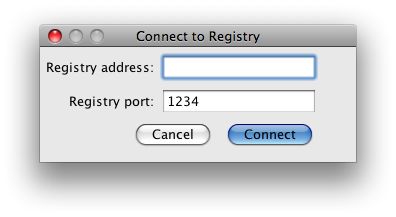
\includegraphics[width=10cm]{gui5.png}
\caption{The dialog for connecting to a rmi registry.}
\label{fig:contoreg}
\end{figure}

If the client is connected to a registry you can create or join groups.

\subsubsection{Creating a group}
To create a group, select Create group from the Group menu. You are now presented with the dialog in figure \vref{fig:creat}. Enter the name of the group and your nickname.

Select group type from the dropdown box, in dynamic groups users can join and leave at anytime, static groups has a fixed set of members.

Choose which type of multicast you would like to use in the group. Basic multicast just sends the messages, reliable multicast guarantees that an attempt to send the message to all users has been made before the message is delivered to the sender.

Finally, select type of ordering and click Create. Please refere to section \vref{messageordering} for descriptions of the available message ordering types.

\begin{figure}
\centering 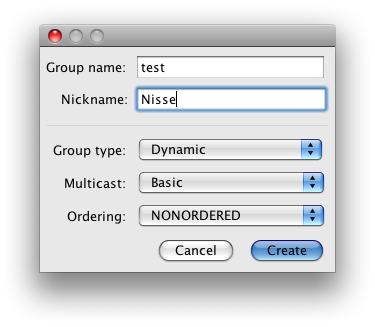
\includegraphics[width=10cm]{gui2.png}
\caption{The dialog for creating a new group.}
\label{fig:creat}
\end{figure}

\subsubsection{Joining a group}
To join a group, select Join group from the Group menu. A dialog like the one in figure \vref{fig:join} is displayed. Enter a nickname and select a group from the Groups list. Do not attempt to join backdoor or sequencer. Click Join.

\begin{figure}
\centering 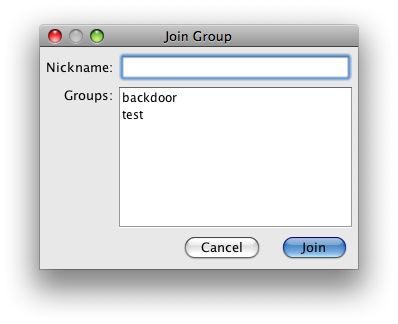
\includegraphics[width=10cm]{gui4.png}
\caption{The dialog for joining a group.}
\label{fig:join}
\end{figure}

\subsubsection{Chatting in a group}
When you have joined a group you will see the group in the tab bar in the main window. Click the groups name to select it (see figure \vref{fig:gui3}). When a group is selected messages from the group is displayd in the big window to the left. To the right a list of members in the group is shown. At the bottom there is a textfield for entering messages to the group. You send a message by pressing Enter in the textfield.

\begin{figure}
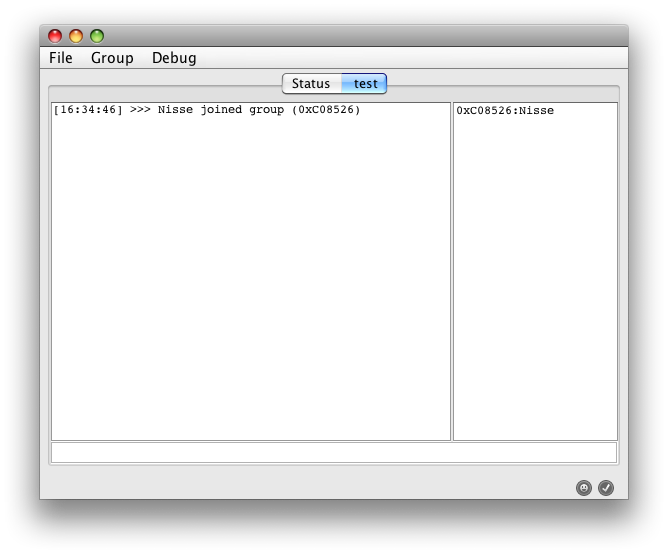
\includegraphics[width=\textwidth]{gui3.png}
\caption{A chat room the user has joined that contains no other users.}
\label{fig:gui3}
\end{figure}


%-----------------------------------------------------------
\section{System Overview}

This project consists of a middle ware for group communication and a demo application to show that it works. The middle ware is located in the gcom and rmi packages, the demo application is in the gui package. An overview over all the packages and their classes can be seen in figure \vref{fig:overview}.

\begin{figure}
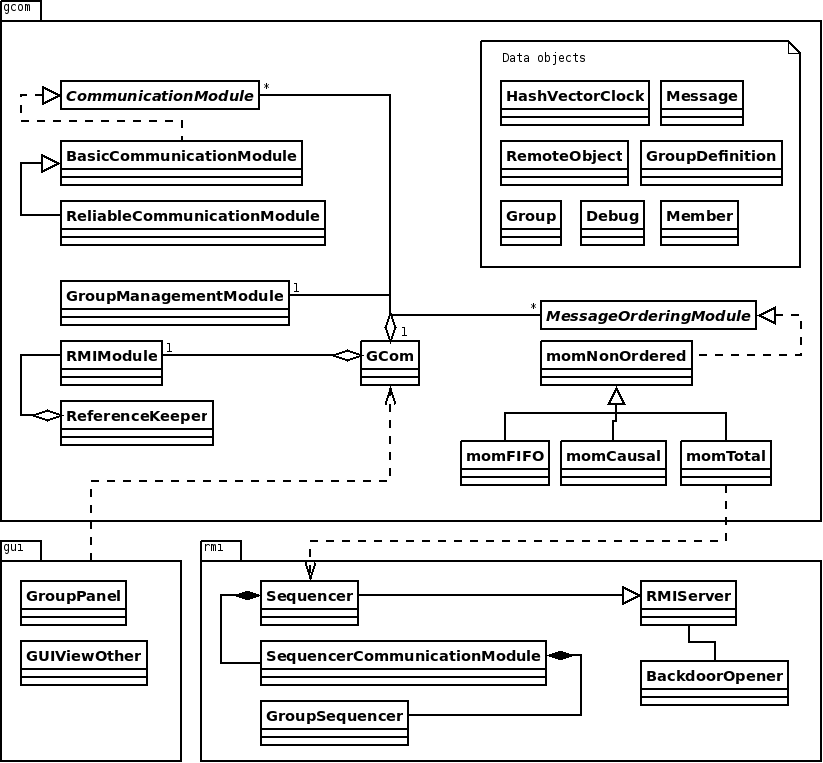
\includegraphics[width=\textwidth]{superuml.png}
\caption{All the classes in the program and an overview of their relations.}
\label{fig:overview}
\end{figure}

\subsection{The gcom package}
The gcom package is the main part of this project. This is where communication, message ordering and group management is handled. 

\subsubsection{GCom}
GCom is the main component in this package and is where the demo application is connected. The application gives commands to GCom, for example create a group or send a message, these commands are translated to messages that GCom sends through the appropriate communication module and to commands to the GroupManagementModule so that the current group state can be maintained.

Information also flows from the communication modules via the message ordering modules back to gcom when messages from other clients is received. These messages either effects the group state or is application data that GCom forwards to the application. 

GCom has one GroupManagementModule, one RMIModule and the same amount of communication and message ordering modules as the number of groups it handles.

\subsubsection{BasicCommunicationModule}
The BasicCommunicationModule (BCM) is the simplest implementation of the interface CommunicationModule. It implements basic multicast and has the ability to send and receive messages. Each communication module corresponds to a specific group. 

When a message is sent the BCM sends it to every member of the group, including the sender. It also detects if the connection is refused to any of the senders and removes these members from the group via a message to GCom.

When the BasicCommunicationModule receives a message the message is sent directly to the message ordering module for the group.

\subsubsection{ReliableCommunicationModule}
The ReliableCommunicationModule (RCM) extends the BCM and implements reliable multicast.

When the RCM receives a message it checks if it has received it before, if not the message is added to a cache of received messages, sent to all group members via BCM and then delivered to message ordering.

Sending messages in the RCM also stores the message in the cache. The message is then sent to all members of the group and the message is delivered to the sender.

When a message is added to the cache, the size of the cache is also trimmed by removing the oldest message if the cache is larger than a specified max size.

\subsubsection{GroupManagementModule}
The GroupManagementModule (GMM) stores information about groups and can notify listeners when something changes.

The main responsibilities for the GMM includes storing group state, resolving group names to members and updating group state when changes are received.

\subsubsection{RMIModule}
The RMIModule connects to a rmi registry at a given host and port. It then supplies an interface for binding, finding, unbinding and rebinding objects.

\subsubsection{momNonOrdered}
The momNonOrdered is the simplest implementation of the MessageOrderingModule (MOM) interface. Every group has a corresponding message ordering module. The type depends on what the creator of the group chose. 

Message ordering is described in detail in section \vref{messageordering}.

\subsubsection{momFIFO}
This message ordering sorts messages in a First In First Out order, in this case this means that messages is delivered in the same order the sender sent them. See section \vref{mo-fifo} for details.

\subsubsection{momCausal}
Causal ordering orders messages according to a happened before relationship. See section \vref{mo-causal} for details.

\subsubsection{momTotal}
Total ordering means that all clients deliver the messages in the exact same order. See section \vref{mo-total} for details.

\subsubsection{ReferenceKeeper}
The ReferenceKeeper is used by GCom only for the group leader. It checks that the rmi registry has the reference to the leaders RemoteObject and tries to rebind it if not. The ReferenceKeeper is run in it's own thread and rechecks the reference in the registry every minute.

\subsubsection{HashVectorClock}
The HashVectorClock implements VectorClock. It stores a clock state with integer values for different process IDs. The clock can be compared to another clock, merged with another clock and ticked, which increases the clock value for the owner by one.

\subsubsection{GroupDefinition}
A GroupDefinition stores information about a group like message ordering, communication type and if the group is static or dynamic. 

\subsubsection{RemoteObject}
The RemoteObject is used for communication between processes via java RMI. 
%TODO: write more about remote object

\subsubsection{Group}
Group stores members and GroupDefinition for a specific group. This class is only used by the GroupManagementModule for storing state.

\subsubsection{Member}
Member stores id, name and RemoteObject for a member in a group.

\subsubsection{Message}
Message is a serializable class used for sending information between processes and modules. A message contains a vector clock, group name, source, message type and message data. Messages used for requesting serial numbers from the sequencer also has a return address.

\subsubsection{Debug}
Debug holds a log4j logger and is used for printing debug and error messages.

\subsection{The rmi package}
The rmi package contains classes related to the rmi registry. 

\subsubsection{RMIServer}
The RMI server creates a registry and opens a backdoor for binding objects remotely.

\subsubsection{BackdoorOpener}
BackdoorOpener is used by RMIServer to create a backdoor. The backdoor is needed since the used implementation of the registry does not allow remote processes to bind objects.

\subsubsection{Sequencer}
The Sequencer is used for getting a serial number on messages that all clients can agree to. There is therefor only one sequencer per group, and in our implementation only one in total.

It extends the RMI-server and therefor first starts a registry. It then binds in a SequencerCommunicationModule SCM as "sequencer" in the registry which the clients that uses any of the total orderings will know that they can connect to. 

Clients can request serial numbers by sending a message to the sequencer and supplying a return address in the message. The Sequencer will order the messages it receives in either a momNonOrdered or a momCausal depending on if total or causal total ordering is requested. Messages that has already been sequenced are cached and the same seri
al number will be returned if a new request for the same message arrives.

\subsubsection{SequencerCommunicationModule}
The SequencerCommunicationModule (SCM) implements CommunicationModule since it makes communication with it convenient, but the module itself is only used by the sequencer. 

It receives messages and returns them to the return address with a serial number. The serial numbers is supplied by a GroupSequencer. Each group has it's own GroupSequencer.

\subsubsection{GroupSequencer}
GroupSequencer (GS) is used by SCM for setting serial numbers on messages. The GS uses a MOM to order the messages before a serial number is given to them. Messages are cached with their serial numbers so requests for the same message gets the same number. 


\subsection{The gui package}                                                                                    
The gui package implements our demo application: a chat application with tabs for groups. 

\subsubsection{GroupPanel}
%TODO: write about group panel

\subsubsection{GUIViewOther}
%TODO: write about gui view other 


%-----------------------------------------------------------
\section{Message ordering and message ordering modules}
\label{messageordering}
GCom features five kinds of message orderings: NonOrdered, FIFO, Causal, Total and CausalTotal. The first four of these has their own message ordering module. Each type of ordering and it's corresponding class is described in detail below.

The message ordering modules have each been thoroughly tested with unit tests to make sure that the algorithms works like intended.

Additional information about algorithms and definitions of the ordering types above can also be found in \cite{distsys-ordering}.

\subsection{Non ordered / momNonOrdered}
The non ordered ordering module (MOM) does not order messages at all. This is the base class for the ordering modules. Every message ordering module has a queuing method, a vector clock and message listeners. All the NonOrdered does is to receive messages in the queue method and send them through to it's messages listeners directly. This is also shown in figure \vref{fig:nonorderd}.

The module also has two functions related to the vector clock. It increases the vector clock when told so and returns the clock values if asked. These functions is used in several of the child modules that inherits from momNonOrdered.

\begin{figure}
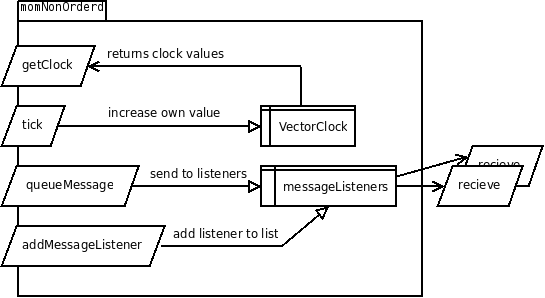
\includegraphics[width=\textwidth]{momNonOrderd.png}
\caption{The non ordered message ordering module just forwards messages to it's listeners. The state of a vector clock is also kept in the module.}
\label{fig:nonorderd}
\end{figure}

\subsection{FIFO ordering / momFIFO}
\label{mo-fifo}
The FIFO ordered MOM delivers messages in the order they where sent. This works by numbering every sent message with a vector clock and storing received messages in a hold back queue until they can be delivered in order. Messages in the queue is compared to the previous last delivered message from the same sender. Messages from new senders is delivered directly as no clock value is known. This is also described in figure \vref{fig:fifo}.

In detail the sorting algorithm works as follows:
\begin{enumerate}
\item Check if no previous messages has been received from this sender, if so:
	\begin{enumerate}
	\item Send message to message listeners.
	\item Increase local clock value for sender by one.
	\end{enumerate}
\item If not, add message to the hold back queue.
\item Loop through the hold back queue and with any message that has a clock value that equals the local clock value plus one:
	\begin{enumerate}
	\item Send message to message listeners.
	\item Increase local clock value for sender by one.
	\item Remove message from hold back queue.
	\end{enumerate}
\end{enumerate}

\begin{figure}
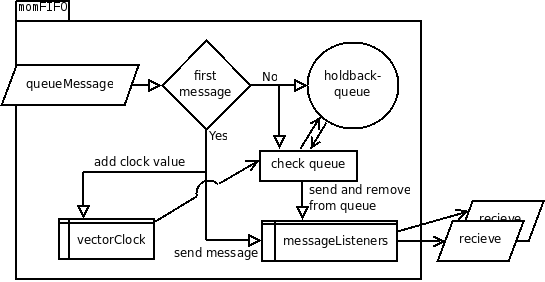
\includegraphics[width=\textwidth]{momFIFO.png}
\caption{The FIFO ordered MOM places messages in a hold back queue until they can be delivered in the order they where sent. Messages from new senders are delivered directly as no previous clock value is known.}
\label{fig:fifo}
\end{figure}

\subsection{Causal ordering / momCausal}
\label{mo-causal}
Causal ordering is an ordering where a message can not be delivered before a message that happened before it. Just like in the FIFO ordering the message is first placed in a hold back queue. If a new sender is detected their clock value is added to the local clock.

Messages in the queue is checked when a message is received. If all previous messages from the same sender has been delivered, and all messages delivered by the sender when the message was timestamped has been delivered, then the message can be delivered. See figure \vref{fig:causal}.

In detail the sorting algorithm works as follows:
\begin{enumerate}
\item Check if no previous messages has been received from this sender, if so:\\
	Add senders clock value minus one, from message to local clock
\item If not, add message to the hold back queue.
\item Loop through the hold back queue and with any message that:
	\begin{enumerate}
	\item Has a clock value for the sender that equals the local clock value for the sender plus one
	\item Has clock values before or equal to corresponding local clock values, excluding the value for the sender
	\end{enumerate}
	Do the following:
	\begin{enumerate}
	\item Send message to message listeners.
	\item Increase local clock value for sender by one.
	\item Remove message from hold back queue.
	\end{enumerate}
\end{enumerate}

In step 1 the clock value minus one is added to the local clock, this is since the message can not be delivered directly like in FIFO ordering (the message might not conform to criteria b). 

\begin{figure}
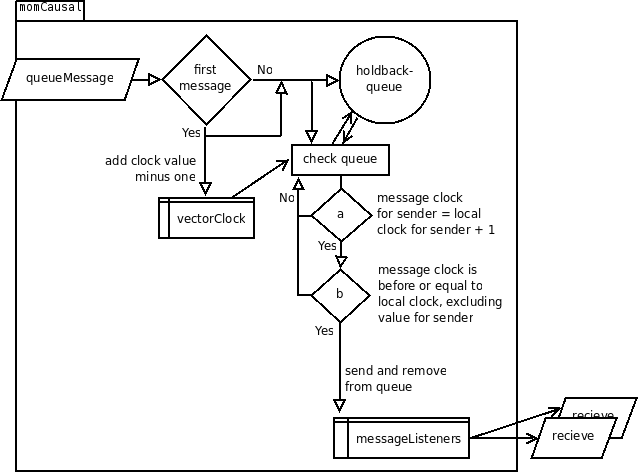
\includegraphics[width=\textwidth]{momCausal.png}
\caption{The Causal ordered MOM places a message in a hold back queue until all messages that happened before it has been delivered.}
\label{fig:causal}
\end{figure}

\subsection{Total ordering / momTotal}
\label{mo-total}
Total ordering is an ordering where every client delivers the messages in the same order. In our implementation this is solved by the use of a sequencer, which is an application that is global for the group. 

When a message is received it is sent to the sequencer. The sequencer gives the message a serial number and sends it back. When the MOM gets a message with a serial number it puts it in hold back queue until it can be delivered in sequence (that is until all messages with a lower number is delivered). This is also described in figure \vref{fig:total}.

The first message with a serial number the MOM receives is delivered directly and any message with a lower number than that is discarded.

\begin{figure}
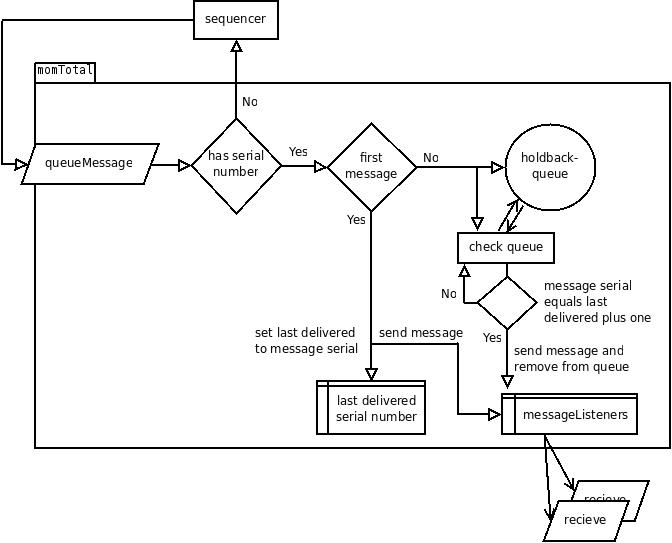
\includegraphics[width=\textwidth]{momTotal.png}
\caption{Total ordering uses a sequencer to deliver messages in the same order in every client.}
\label{fig:total}
\end{figure}

\subsection{Causal total ordering}
Causal total ordering uses the same MOM as total ordering. The only difference is in the sequencer.

With causal total ordering the sequencer uses a momCausal to order the messages in causal order and gives them serial numbers in the order they are delivered. This interaction is shown in figure \vref{fig:totalc}.

\begin{figure}
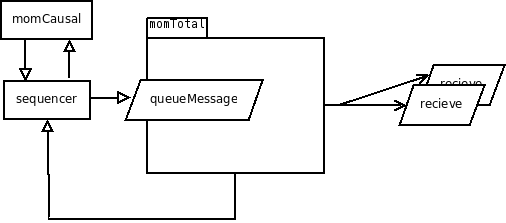
\includegraphics[width=\textwidth]{momTotalC.png}
\caption{Causal total ordering also uses a sequencer, but here the sequencer has a MOM of it's own to give the messages serial numbers in causal order.}
\label{fig:totalc}
\end{figure}

%-----------------------------------------------------------
\section{Design decisions}

\subsection{Selection of bonus level}
We chose to solve bonus level two with dynamic groups since if seemed like an reasonable trade off between extra credits and extra workload. 

\subsection{Why an chat Application?}
As our demo application on top of gcom we built a chat application with tabs for different groups. This type of application maps well to the underlying structure of members that belongs to groups. It also gave an easy way to see that messages arrive unharmed and in the correct amount. 

\subsection{Why using a sequencer for total ordering?}
When implementing total ordering one can either use a sequencer or a distributed algorithm. The sequencer method has the downside of the sequencer being the single point of failure. However we still choose that method since it seemed more straightforward to implement and we already had a single point of failure.

\subsection{Why the sequencer lives in the rmi-server}
The RMI-server has to be started before the sequencer and we only wanted a single instance of both so it made sense to put them in the same module (or rather, make the sequencer extend the RMI-server). The RMI-server is also a hopefully quite stable host which makes it a good location for the sequencer.

It would have scaled to more users to put the sequencer in the group leader, but this would make the sequencer less stable (since the group leader might choose to leave the group).

An obvious drawback of having a single sequencer for all groups is that it becomes a bottleneck. This could be solved by moving the sequencer to several dedicated hosts and assigning groups to one of many sequencers.

%-----------------------------------------------------------
\section{Fault tolerance}
\subsection{Detecting crashed members}
The communication module detects if a client refuses connections or if connections timeout. If this happens the member is removed from the group management module and a lost member message is sent.

If the crashed client is the group leader a new leader is elected.

\subsection{If the registry restarts or is unresponsive}
The leader of each group occasionally checks that the group is registered in the RMI-registry. If the registry has restarted for some reason the leader will re-register the group.

\subsection{If the group leader crashes}
If the group leader crashes the group will detect that no messages arrive from the leader and then elect a new leader. 

\subsection{Election of a new leader}
%% TODO: Write about election algorithm

\subsection{If the last member of a group crashes}
If the last member of a group crashes no one will unregister the group.
This will potentially lead to a lot of "dead" references in the registry if there is a bug causing nodes to crash when they are the last to leave a group. In order to counter this extra testing has be done to make sure that nodes behave when leaving and unregistering with the registry.

There is currently no way to clear out old references in the registry (other than restarting it periodically).

\subsection{Netsplit}
If the group is split in two partitions, due to a cable failure or similar, the partition with the leader will continue to work as before. The other partition will elect a new leader when they discover that they no longer receive messages from the leader.

The new leader will try to reregister the group in the registry. The leader for the other part will do the same and therefore compete over the reference in the registry. Because of this newcomers will join the group having the reference in the registry at the time the node connects.

\section{Realization of the project plan}
The project plan from deliverable 1 is included in appendix \vref{app:projectplan}. We have been slightly behind the plan during most of the project part due to the new influenza that struck Emil during one of the first weeks.

We also moved forward the design of the GUI to milestone 4 since it was easier to do while implementing the actual application. We also moved total and causal total ordering forward one week since the other message orderings took most of the assigned week. 

Generally things took slightly longer then anticipated, part due to tricky bugs and part due to tricky algorithms. 

%-----------------------------------------------------------
\section{Implementation of requirement specification}
Below our requirement specification from out project plan is included in appendix \vref{app:reqspec}. We have succeeded with implementing all required specifications. 

%-----------------------------------------------------------
\section{Limitations}
\begin{itemize}
\item The RMI-registry is a single point of failure. If the registry crashes no processes can find or join groups until the registry has been restarted.

\item If a group is split in two parts due to network failure and both parts still have contact with the registry bad things will happen. This is assumed to never happen.

\item All processes are assumed to be good. If a process starts to lie or send malicious messages bad things will happen.

\item If a client crashes during election undefined things happen.

\item If the sequencer crashes all groups using the sequencer must be restarted since the message cache is lost and messages will get new serial numbers starting at 1. The sequencer is placed at the same host as the registry which is assumed to be relatively stable for this to not be a big problem.

\item If a group contains too many users java will run out of memory and the client will crash. If reliable multicast is used the network will most likely also be very congested.

\item The demo application does not use the remove group feature of GCom since it is more user friendly to let the group live as long as there is users conencted to it and remove it when the last user quits. However, the feature is implemented and can be used by some other application that uses the middle ware.

\item The program does not build under Windows. Usage of windows is discourage and behaviour is undefined.

\item In the demo application backdoor and sequencer is visible in the groups list.

\end{itemize}

\begin{thebibliography}{5}
\bibitem{distsys-ordering} Distributed systems : concepts and design / GeorgeCoulouris, Jean Dollimore, Tim Kondberg.--4th ed. p. 490-498

\end{thebibliography}

\appendix
\section{Project plan}
\label{app:projectplan}
\begin{tabular}{|l|l|p{7.5cm}|}
\hline
Date	&	Milestone	&	Content \\
\hline
11 Sept	&	Part 1 due	&	Written project plan \\
18 Sept &	Milestone 1 &	Create all interfaces \\ 
						&&	Build dataobjects \\
						&&	Design GUI mockups for test app \\
25 Sept &	Milestone 2 & 	Implement basic methods like non-ordered ordering and non-reliable multicast. \\
2 Oct	&	Milestone 3 & 	Implement advanced methods like total ordering and reliable multicast. \\
9 Oct	&	Milestone 4 & 	Implement GUI-application and debug mode. \\
16 Oct	&	Milestone 5 & 	Resolve distributed problems. \\ && Write on the report.\\ && Make test protocol. \\
23 Oct	&	Finalization 	& Everything should be finished. Minor adjustments. \\
27 Oct	&	Hand in report 	& \\
28-30 Oct & Demonstration	& \\
\hline
\end{tabular}

\section{Requirement specification from project plan}
\label{app:reqspec}

\subsection{Group management}
\begin{description}
\item[REQUIRED] External processes must be able to find and connect to group leaders via a RMI registry.

\item[REQUIRED] The group leader must regularly make sure that the group and leader is registered in the RMI registry.

\item[REQUIRED] Any process must be able to create a new group and register itself as leader in the registry.

\item[REQUIRED] Any process must be able to join a group by connecting to the group leader.

\item[REQUIRED] Every process in a group must notify the other processes of any known changes to the group composition.

\item[REQUIRED] Every process must keep track of the members of all the groups it's a member of.

\item[REQUIRED] Every process must monitor if another process in the group stops responding and report a corresponding change in group composition.

\item[REQUIRED] If the leader of the group leaves or crashes a new leader must be elected in the group.
\end{description}


\subsection{Communication}
\begin{description}
\item[REQUIRED] It must be possible to send messages to the members of joined group.

\item[REQUIRED] Both non-reliable and reliable multicast must be supported for sending messages.

\item[REQUIRED] The communication method chosen by the group creator (reliable or non-reliable multicast) must be used when communicating in a group.

\item[REQUIRED] Every message must contain a updated vector clock.
\end{description}


\subsection{Message Ordering}
\begin{description}
\item[REQUIRED] Any message must arrive in proper order (according to the selected sorting requirements).

\item[REQUIRED] A message must not be delivered until all previous messages are delivered if the message ordering demands so.
\end{description}




\end{document}
